\chapter{System Architecture}\label{cap:development}
In this chapter, the architecture and structure adopted for the construction of the system components are discussed in detail. It is important to understand that the system was conceived as a set of modules, with each one performing specific functions, and when operated together, these modules result in the achievement of the purposes intended for the system.

The system is fundamentally structured in distinct layers, the backend, the frontend, and the database.

\begin{figure}[htbp]
	\centering
	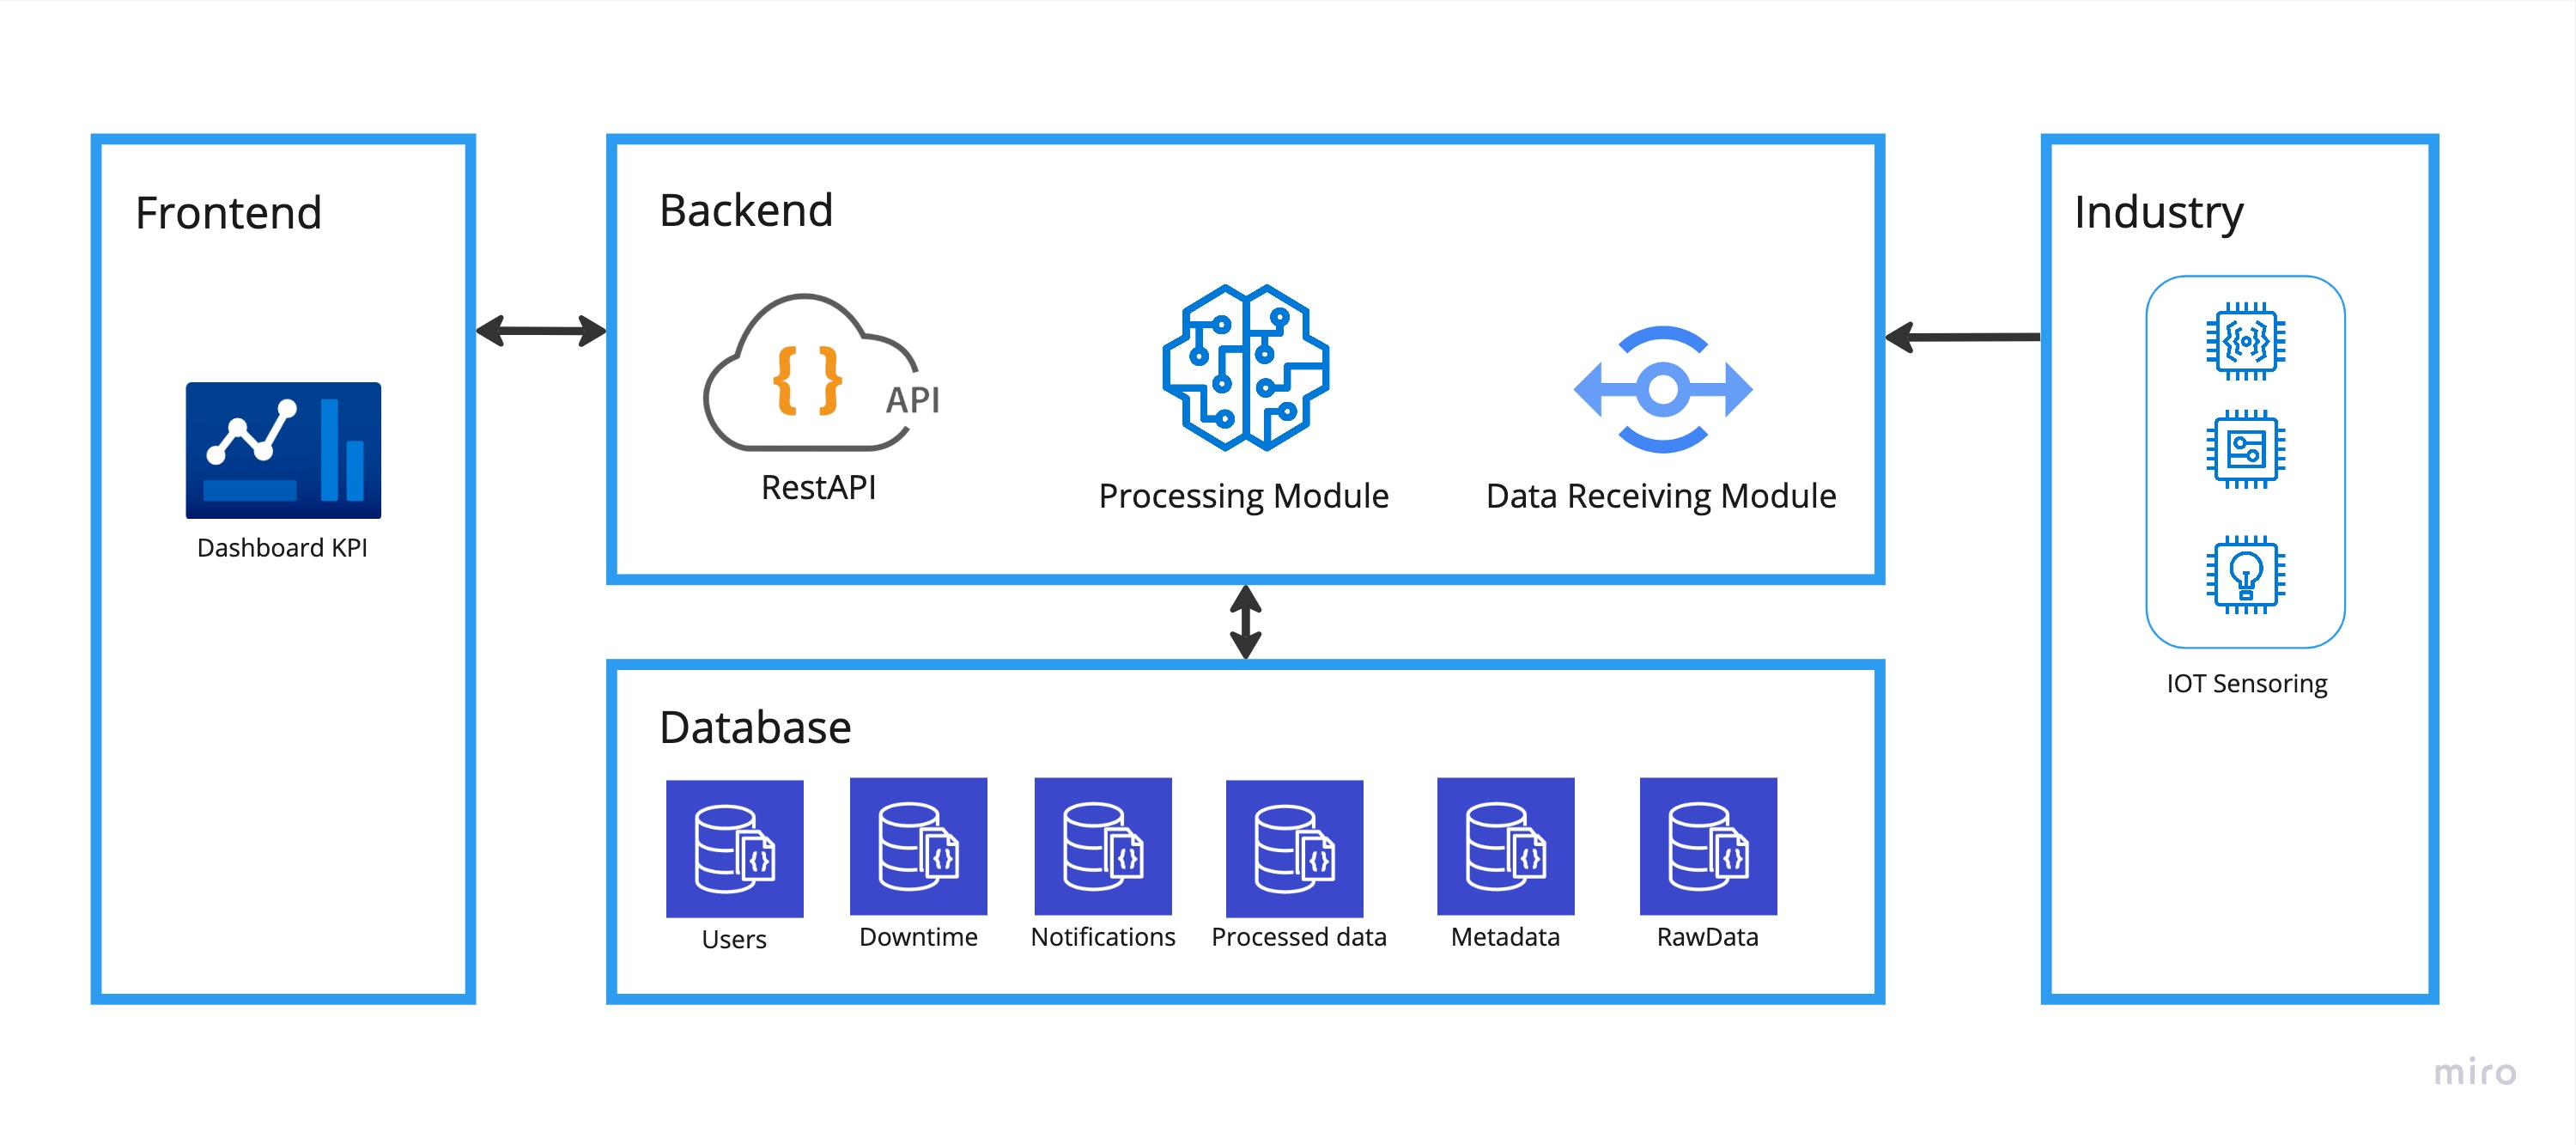
\includegraphics[width=\textwidth]{images/Architecture.jpg}
	\caption{System architecture.}
	\label{fig:systemAchitectureImage}
\end{figure}

The backend functions as the core of the system. Its main role is to receive the data, process it according to the rules established in the requirements and user stories, and store it securely in the database. In addition to storage and processing functions, the backend is also assigned the responsibility of making these data available through an \gls{API}, which can be accessed using \gls{HTTP} methods. This \gls{API} acts as an intermediary between the central logic of the system and the interfaces with which the end user interacts, the frontend.
On the other hand, the frontend is characterized as the visual interface that the end user accesses. It serves as a means by which users interact with the system, sending and receiving information. This layer is designed to access, retrieve, and present the data processed and stored by the backend according to design principles and data visualization \cite{barbosa2019introduction}.

As can be seen in figure ~\ref{fig:systemAchitectureImage}, in the industrial plant, where the machines with the sensors are located, the sensors send the data to the system, which receives them through the data receiving module and stores them in the database. The processing module accesses the stored data to perform aggregation, and the \gls{API} manages access to the database, making the information available to users on the frontend.

In the following sections, each of these components will be explored more deeply, going through their specificities and interactions.


\section[Backend Architecture]{Backend Architecture}
This section addresses the operation of the backend. It is divided into three parts, the module for receiving data from the sensors, the processing module where the aggregation and statistical analysis of the data is done, and the \gls{API} that manages access to information through \gls{HTTP} requests.

Regarding the organization of the repositories, the \gls{API} and the data receiving module are in the same repository, facilitating communication between them. The processing module, on the other hand, is in a separate repository, its only function being to read the database, process the data, and store the results.

\subsection{Data Receiving Module}\label{subsec:receiveDataModuleArch}
For the data receiving module, initially, the \texttt{SensorConnection} class stands out, whose function is to manage and maintain the connection with the sensor network. This class transmits the received data to a designated function \texttt{save\_data\_func}, ensuring that the data is forwarded for appropriate handling.

In the next part of the architecture, the \texttt{IotSensorConnection} class is used, which originates from the \texttt{IotSensorConnectionInterface} interface. This interface was created to ensure the system's adaptability, facilitating the integration of different types of data receipts, such as a class intended to generate sensor data in a development environment, where there is no access to the real sensor. The \texttt{IotSensorConnection} class, when instantiated, is responsible for establishing the connection, and creating a new thread that operates as an active listener, monitoring the arrival of new information. Upon noticing the reception of new data, the class directs this information to a third entity, which holds the responsibility of applying the business rules.

This third entity is the \texttt{SensorsRepository} class, which, when triggered with data from the sensors, has the responsibility to evaluate the information based on the established parameters, deciding whether it is necessary to trigger an alert, and make the sensor data accessible via \gls{API}, ensuring that these data are available to be transmitted in real time, via stream, to all connected users. Furthermore, the data is saved in the database, specifically in the raw data collection of the data lake, \texttt{Raw Data}. Once saved in the database, these raw data are available to be processed by the processing module.

The data provision by the \texttt{SensorsRepository} class occurs through the instance of the \texttt{SensorValue} class, which with the \texttt{update\_current\_sensor\_value} method updates the data in memory that are accessed by the connected users.

The diagram showing the organization of these classes can be seen in figure ~\ref{fig:receiveData}. This design ensures that the raw data from the sensors are effectively received, evaluated, and stored.

In chapter~\ref{cap:implementation}, the implementation details of this module are further elaborated.


\begin{figure}[htbp]
	\centering
	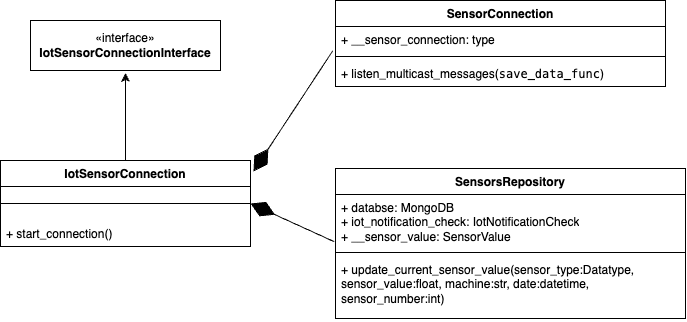
\includegraphics[width=\textwidth]{images/recebimento_dados.png}
	\caption{Module to receive sensor data.}
	\label{fig:receiveData}
\end{figure}


\subsection{Data Processing Module}\label{subsec:moduloProcessamento}
The data processing module was developed to ensure that the raw data collected are processed, providing the statistical analysis that is displayed to the users.

The code is executed when a specific function is invoked, which is responsible for performing a series of operations. Firstly, a list is constituted containing the database collections responsible for storing both the raw data and the already processed data. Simultaneously, a second list is generated, representing the machines that sent information to the system.

With these lists, an iterative procedure begins, in which, for each identified machine, the available data are read, submitted to a statistical analysis process, after which the results obtained are recorded in the processed data collection. This statistical analysis adopts the Box Plot method.

The Box Plot, also known as a box diagram, is a graphical tool used to represent the variation of observed data from a numerical variable through quartiles. In figure ~\ref{fig:boxplot}, the rectangle formed by the first quartile (Q1), median, and third quartile (Q3) can be seen, which provide a notion about the centrality and dispersion of the data, while the "antennas" extend to show the full range of the data, thus helping in the identification of possible outliers.

By adopting the Box Plot, the system ensures a robust understanding of the data distribution, identifying not only central trends but also variations and potential anomalies \cite{marmolejo2010shifting}.

\begin{figure}[htbp]
	\centering
	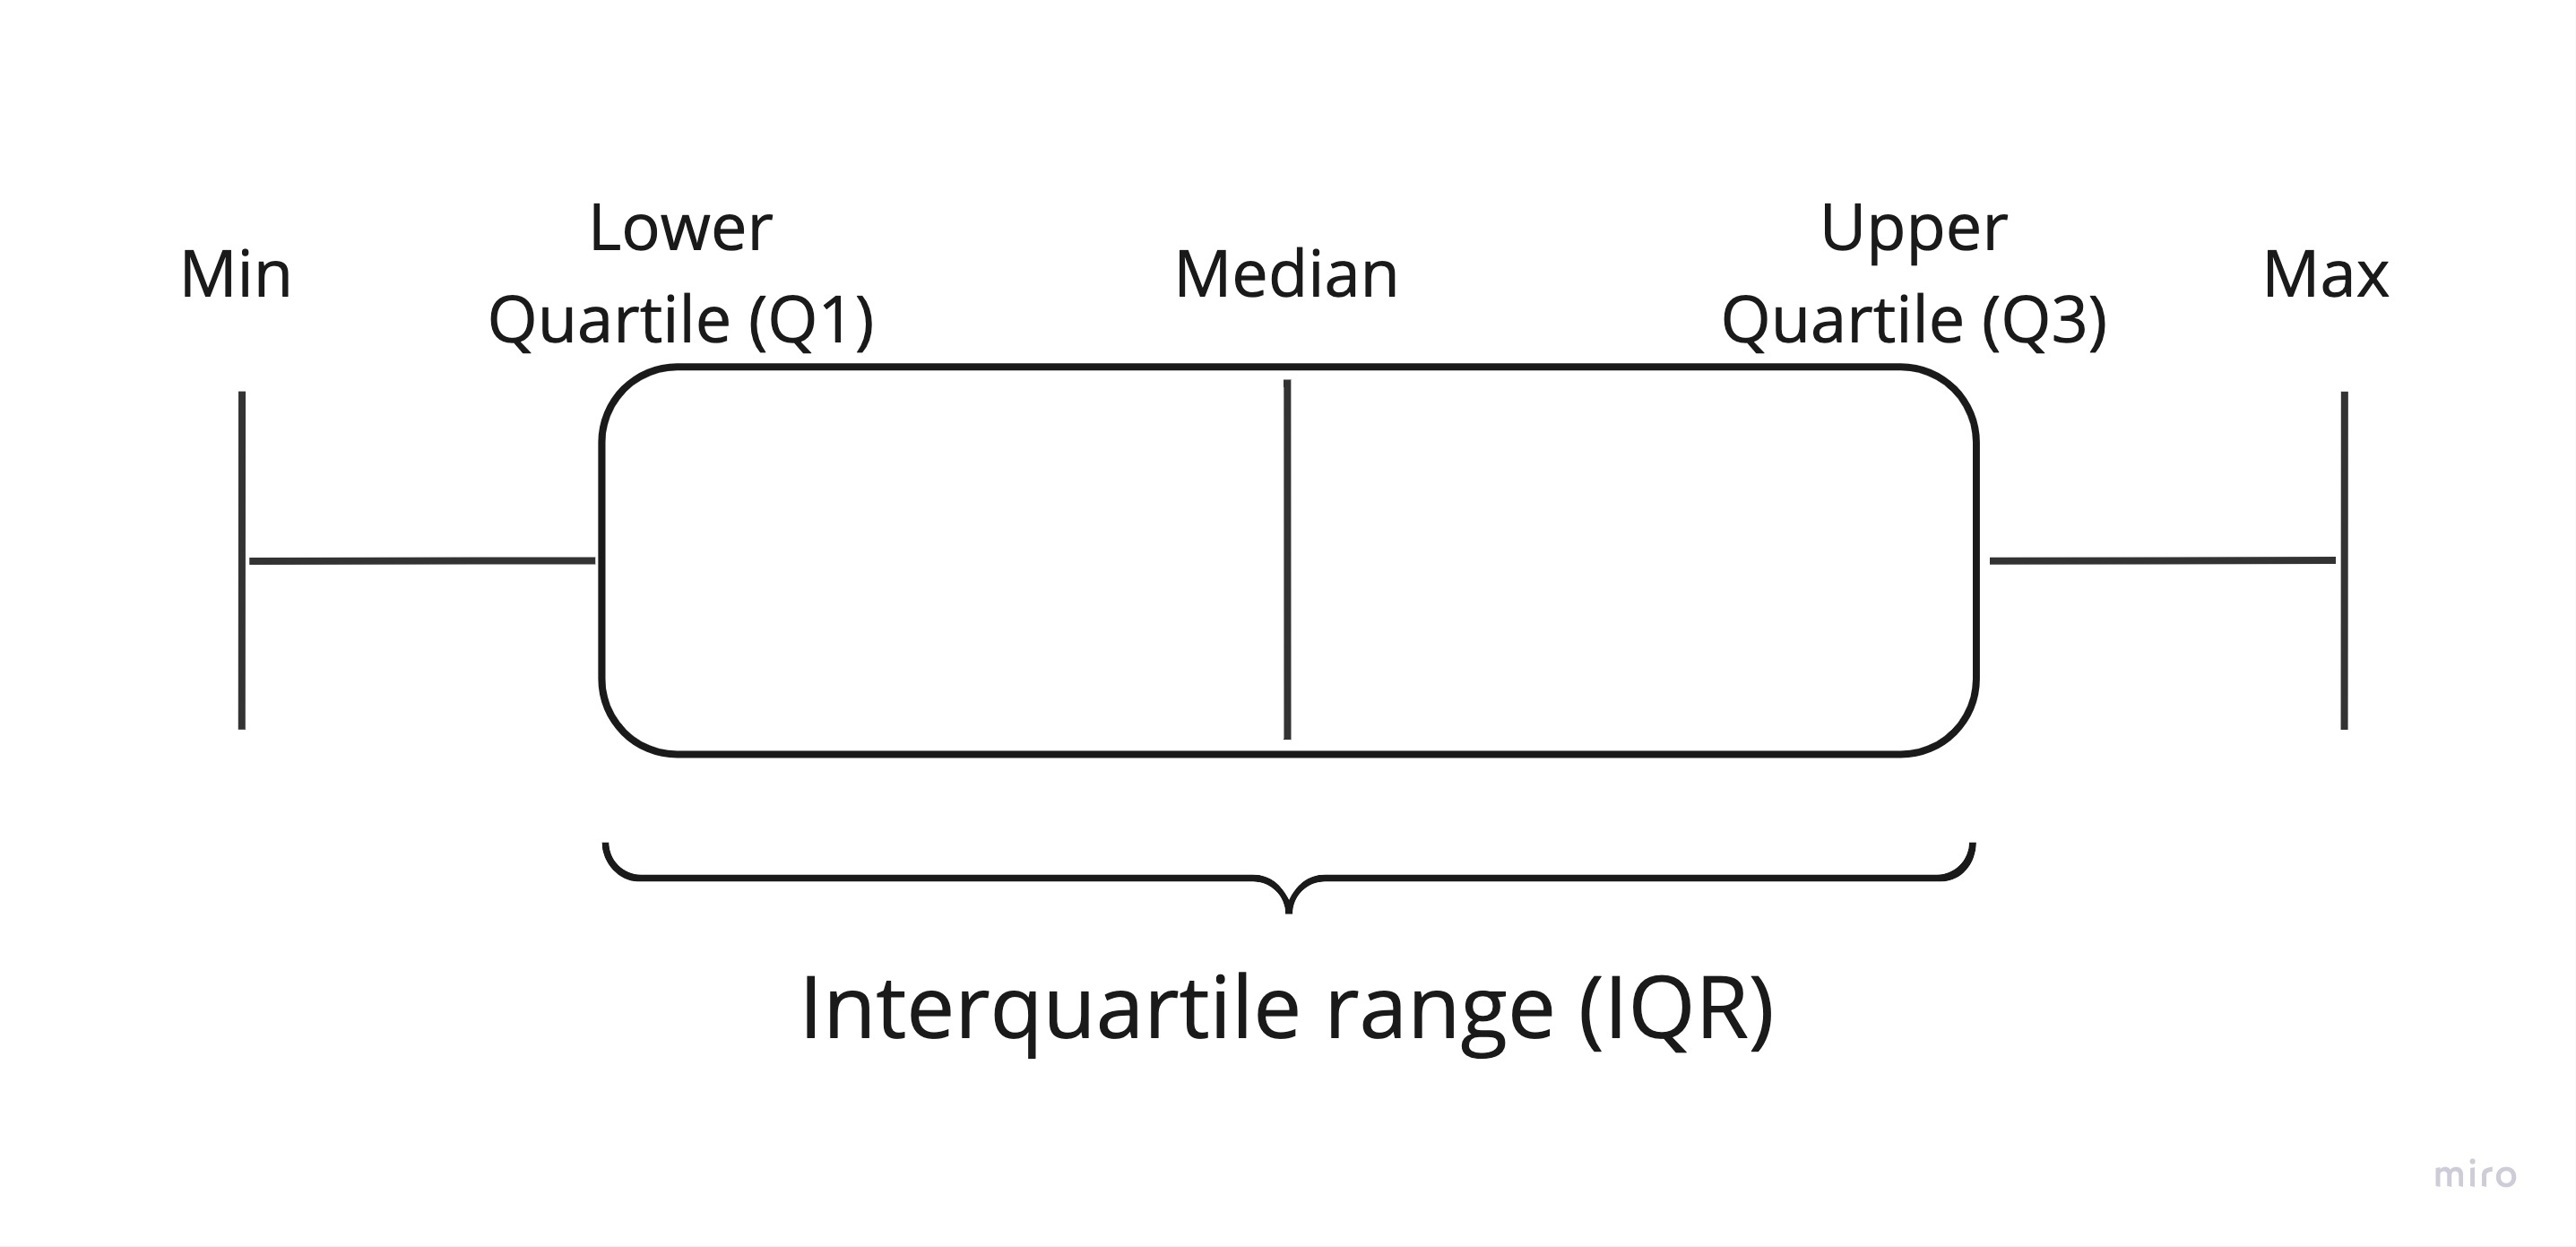
\includegraphics[width=\textwidth]{images/boxplot.jpg}
	\caption{BoxPlot.}
	\label{fig:boxplot}
\end{figure}


\subsection{API}\label{subsec:apiArchitecture}
The \gls{API} was structured into small sub-modules, each focused on a specific context. This modularization ensures that each part of the \gls{API} has a single responsibility. In each module, there is a segmentation composed of: the \textit{controller} layer, intended to receive and manage \gls{HTTP} requests; the service layer, which serves to process the information and apply the respective business rules; and the repository layer, whose role is to establish a bridge with the database, accessing and providing the necessary data. Figure ~\ref{fig:api_organization} represents the folder organization that was used for this architecture.

\begin{figure}[htbp]
	\centering
	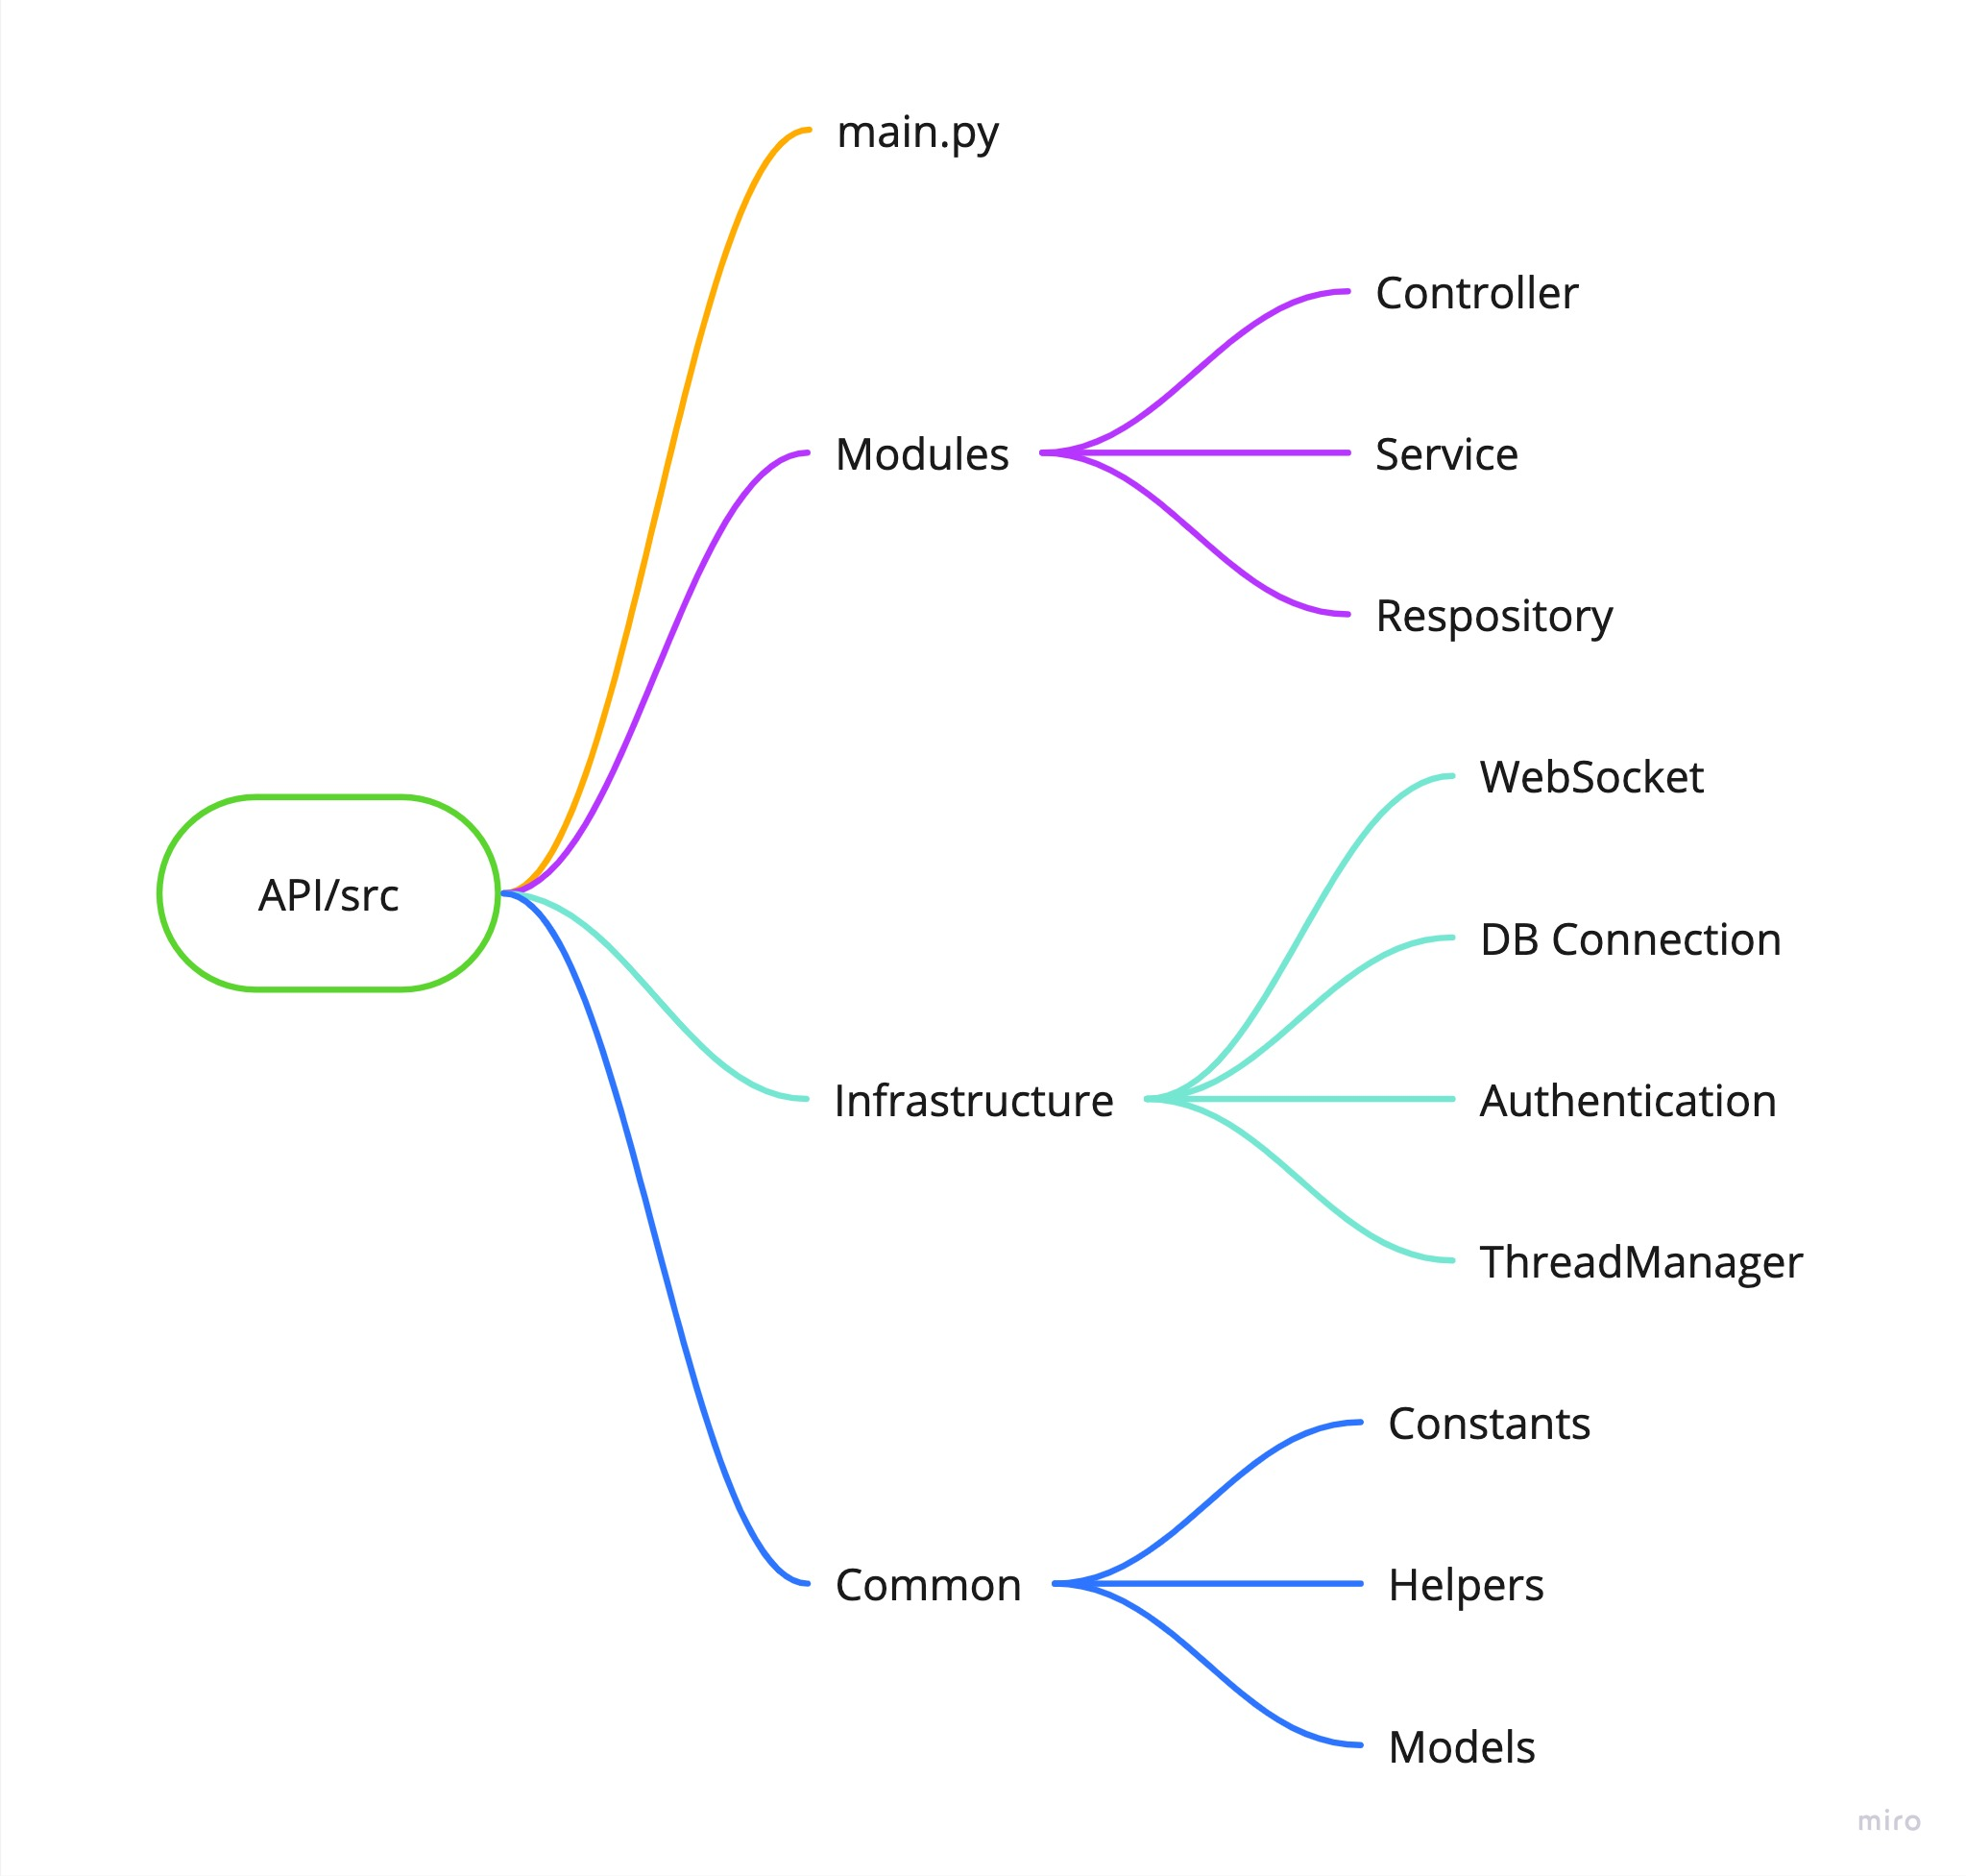
\includegraphics[width=\textwidth]{images/API_Organization.jpg}
	\caption{API Organization.}
	\label{fig:api_organization}
\end{figure}

When a request is sent to the \gls{API}, the first interaction occurs with the controller layer. Once received, this request is directed to the service layer, where business rules are applied. The service layer communicates closely with the repository layer, which holds the responsibility of accessing the database and bringing accurate information, suitable for the demands of the module in question.

The modules implemented in the \gls{API} with the described logic are:
\begin{itemize}
	\item \textbf{Downtime:} Responsible for managing access to downtime data stored for testing in the system.
	\item \textbf{IOT Sensors:} Responsible for managing access to data related to the factory machine sensors.
	\item \textbf{Notification:} Responsible for managing access to notifications generated by the system, as well as web socket connections for sending notifications.
	\item \textbf{User:} Responsible for managing access to user data, as well as performing login and logout operations. 
\end{itemize}

In addition to these modular layers, there is a specific area in the \gls{API} for storing codes common to all modules. This section encompasses various useful functions, class templates, constant values, and default settings. These elements ensure greater cohesion and reduce code repetition, optimizing overall performance. Among the default settings, the initializer that establishes access to the database, authentication middleware, web socket connection for sending notifications, and the initializer of new \textit{threads} deserve special mention. The latter is used for asynchronous operations that are executed in parallel to the operation of the \gls{API}, such as those executed by the data reception module.

\section[Frontend Architecture]{Frontend Architecture}\label{sec:archFront}
Using \textit{Next.js} \cite{nextjsDocs} as a framework, the frontend follows a basic structure already established by it.

The system's routes reside in the \texttt{pages} folder, aligned with the framework's guidelines. The layouts that serve as a base for each page are located in the \texttt{layouts} folder.

\textit{React} components \cite{reactDocs} are the foundation of each page and layout and are organized in a specific layer, allowing them to be reused in various parts of the application.

With the adoption of \textit{Typescript} \cite{typescriptLang}, models define the types of data structure used. These are kept in the \texttt{types} folder, establishing data format contracts for the frontend. This minimizes errors and enhances efficiency in development.

The React \textit{Context API} is used to manage data in components, allowing for centralized sharing of information, as can be seen in figure ~\ref{fig:FrontendOrganization}. This approach optimizes the way data is accessed and distributed in the system, enhancing the organization of the architecture.

\begin{figure}[htbp]
	\centering
	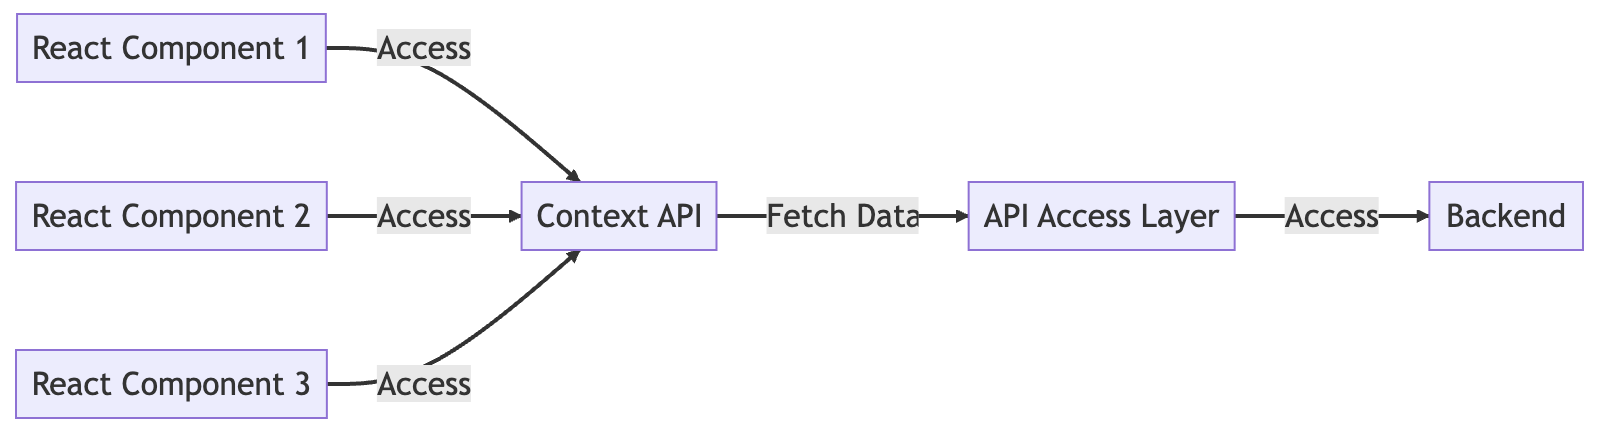
\includegraphics[width=\textwidth]{images/components_frontend.png}
	\caption{Frontend organization.}
	\label{fig:FrontendOrganization}
\end{figure}

There is a specific layer for external access, which manages communication with the \gls{API} and WebSocket connections. This is accessed only by contexts for updating and retrieving data.

Finally, there is a dedicated folder to store recurring codes, containing helper functions, themes, and assets, facilitating development and maintenance by providing a clear and cohesive structure.


\section{Containers}
Containers are technologies that allow applications to be isolated in specific environments with all their dependencies, libraries, and necessary configurations, without the overhead of full virtual machines. This ensures that the application works identically in different environments, from development to production \cite{paraiso2016model}. In figure ~\ref{fig:container}, it is possible to visualize how containers work within the host operating system.

\begin{figure}[htbp]
	\centering
	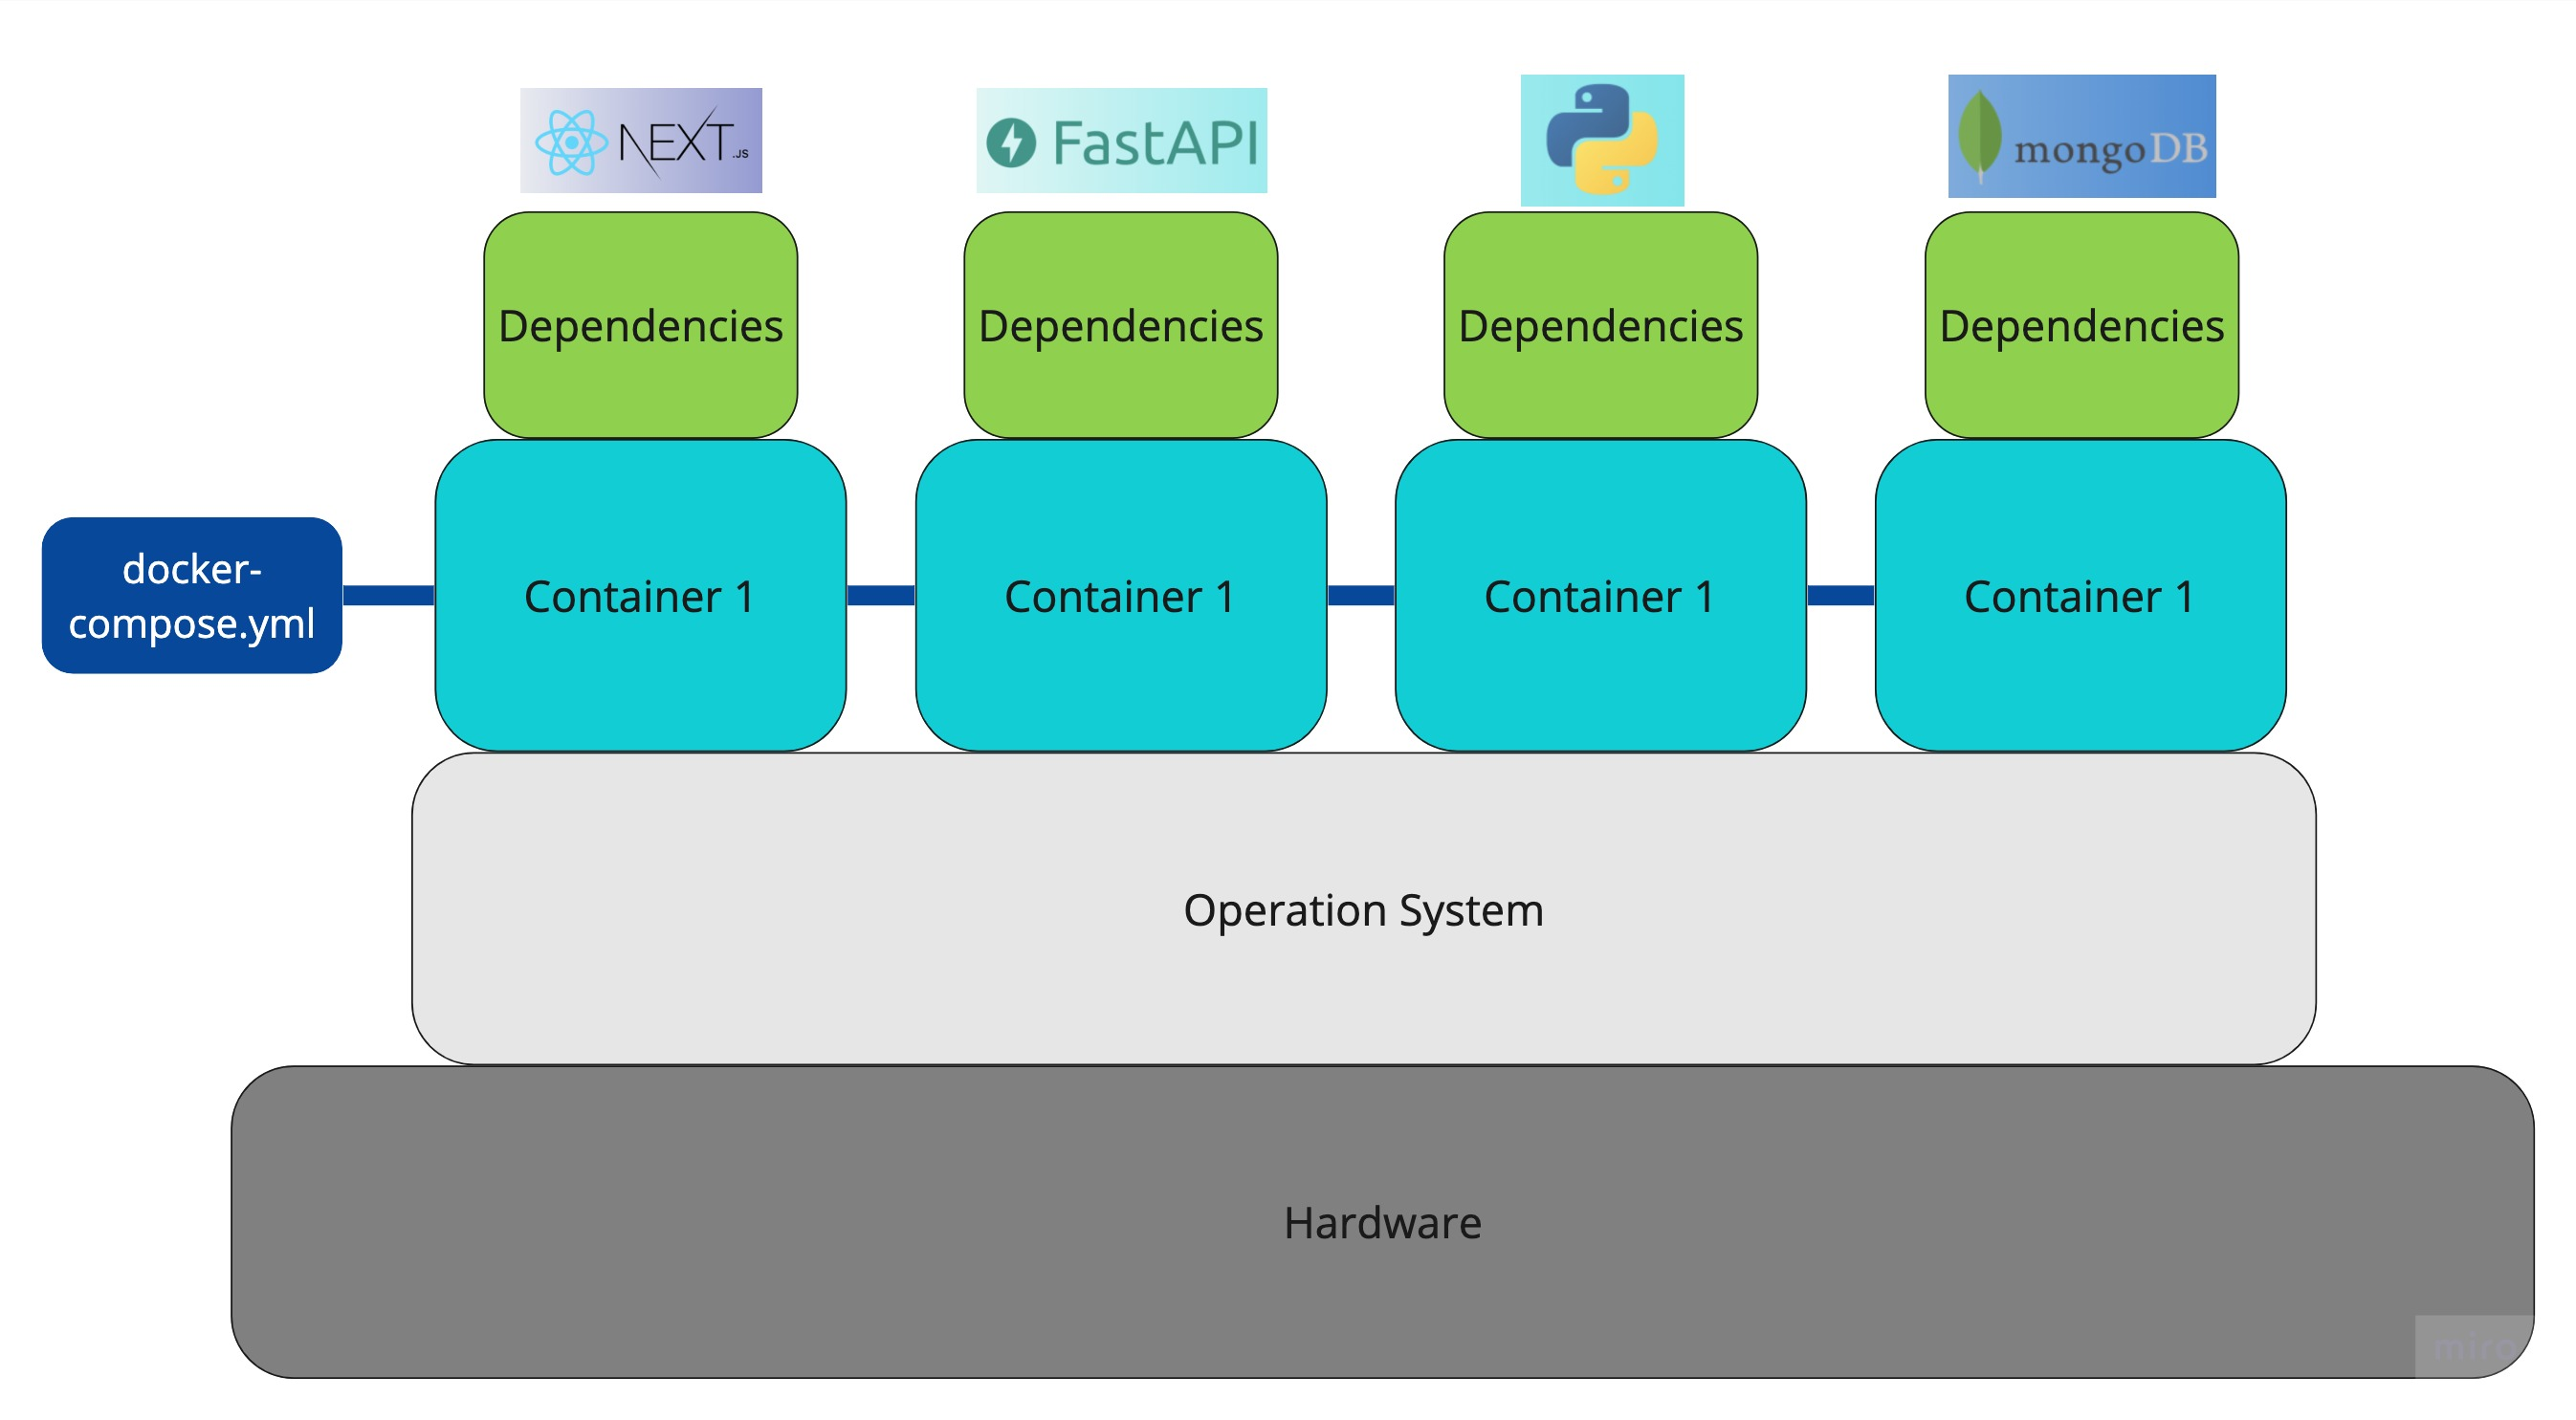
\includegraphics[width=\textwidth]{images/container.jpg}
	\caption{How container works.}
	\label{fig:container}
\end{figure}

Within the universe of containers, \textit{Docker} \cite{dockerDocs} was the tool selected for this project. Several factors influenced this decision, including comprehensive documentation, an active community, and the presence of a wide variety of available content. In addition, Docker simplifies the definition, creation, and execution of containers, making it a robust solution for application deployment.

The system adopts some containers to organize and manage the various parts of the application:
\begin{itemize}
    \item \textbf{Frontend}: A container dedicated to the frontend, built with \textit{NextJs}.
    \item \textbf{Backend}: Divided into two distinct containers:
	\subitem One that encompasses the \gls{API} and the data receiving module;
	\subitem And another one specifically aimed at the data processing module;
    \item \textbf{Database}: A container for the MongoDB database, ensuring isolation and efficiency in data management.
\end{itemize}

The communication between the containers is made possible through a bridge network provided by Docker \cite{dockerNetwork}. This network is a software interface created on the host that allows containers to communicate with each other and with the host, ensuring the necessary connectivity between the different modules of the application. This adds an extra layer of security to the application, as all external connections must be made through this network. The connection with the external network is made through a web server, explained in section ~\ref{sec:webserver}.

To ensure data persistence and prevent the loss of vital information, the concept of Docker \textit{volumes} \cite{dockerVolumes} was employed in the system architecture. Volumes are designated spaces in the host system that can be accessed and used by containers. In the context of this project, a volume was specifically configured for the MongoDB database. Thus, even if the database container is restarted or removed, the database remains intact and available, due to its storage in the volume, which operates independently of the container's lifecycle.

With the need to manage multiple containers, network configurations, and volumes in a cohesive and simplified manner, \textit{Docker Compose} \cite{dockerCompose} was adopted in the system architecture. Docker Compose allows the definition and execution of multi-container applications using a YAML file \cite{yamlOrg}. This file contains all the necessary configurations to initialize and interconnect the containers. Thus, instead of executing a series of commands to start each container individually, it is possible, through Docker Compose, to start the entire system with a single command. This approach not only simplifies the deployment and development process but also ensures that network and volume configurations are consistently applied in each execution.

The use of containers in the project brought advantages. Firstly, it ensured consistency between development and production environments. Additionally, the modularization provided by the containers facilitates the scalability and maintenance of the system, allowing updates and changes to be made quickly and safely as the system grows. Lastly, the use of containers facilitates the portability of the system, which can be run on various types of servers and systems, provided that docker is installed.


\section{Web Server}\label{sec:webserver}

Within the proposed architecture, with containers running different parts of the application, \textit{NGINX} \cite{nginxDocs} was used to intermediate the traffic of requests, ensuring the correct distribution of requests to each container.

The method employed for this is the reverse proxy. In simple terms, the reverse proxy acts as an interface between the client and several servers, directing client requests to the appropriate server (in the context of this project, the containers), thus optimizing resource use and ensuring a faster and more efficient response.

Regarding specific requests, those that involve return in stream format or establish a \textit{WebSocket} connection, specific settings were made in the \textit{NGINX} configuration, these are detailed in chapter~\ref{cap:implementation}, dedicated to implementation. Upon receiving a request, the \textit{NGINX} server identifies, based on it, which container is responsible for the service. After this identification, the appropriate settings are applied, and the request is directed to the corresponding container to obtain the response. This workflow can be seen in figure ~\ref{fig:nginx_workflow}.

\begin{figure}[htbp]
	\centering
	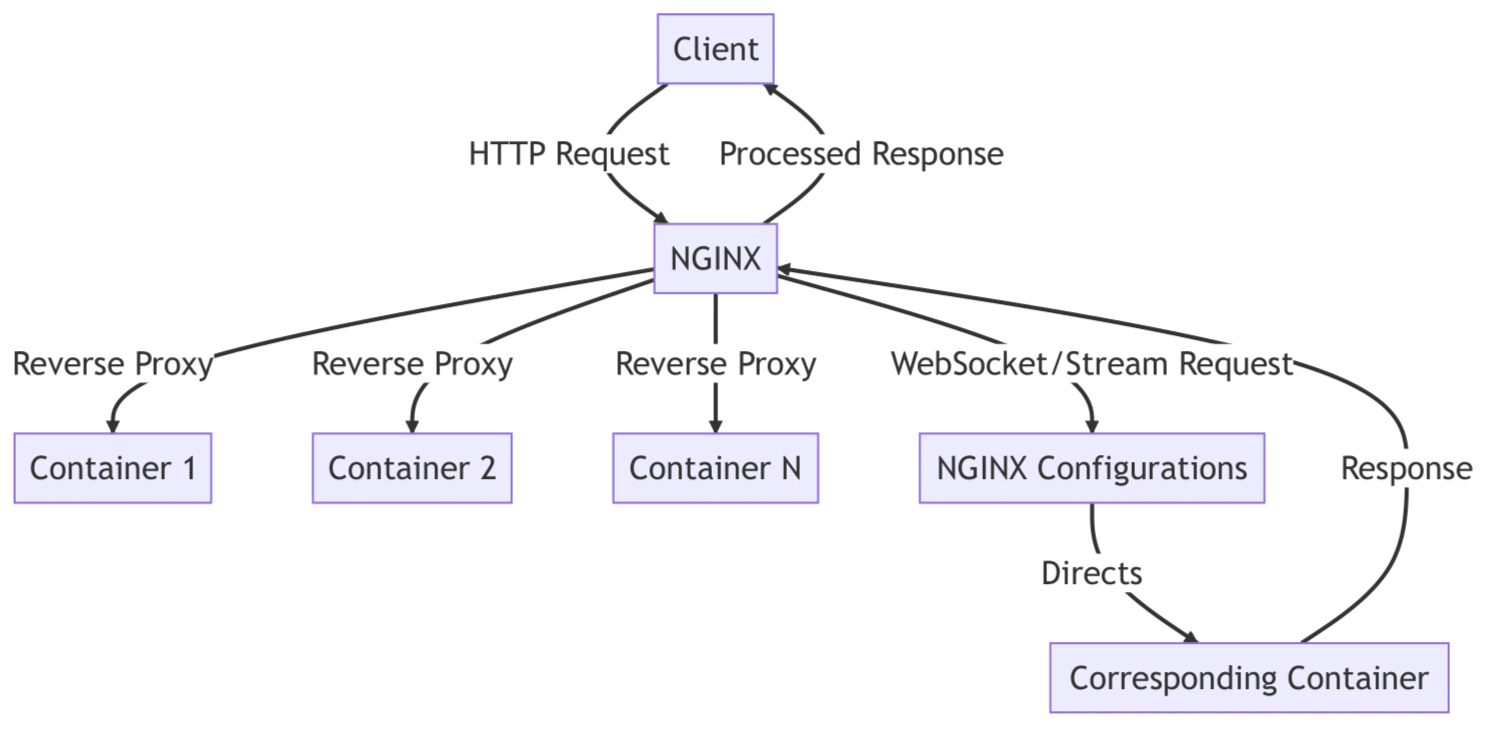
\includegraphics[width=\textwidth]{images/diagrama_nginx.png}
	\caption{NGINX workflow.}
	\label{fig:nginx_workflow}
\end{figure}

The incorporation of \textit{NGINX} brought some benefits to the project. One of them is the additional layer of security: \textit{NGINX} limits direct access to the containers, serving as a barrier against unauthorized access attempts. Additionally, with NGINX, the scalability process becomes simpler and more efficient, thanks to the server's inherent ability to act as a load balancer. This load balancer distributes incoming traffic among several servers, ensuring that no server becomes overloaded. This feature not only improves overall performance but also provides greater system availability, as in the event of a server failure, traffic can be directed to another operational one.